
%author: Ricardo Soto [ricardo.soto@ucv.cl]

\documentclass[11pt]{article}
\usepackage[english]{babel}
\usepackage[T1]{fontenc}
\RequirePackage[a-1b]{pdfx}
\usepackage[latin1,utf8]{inputenc}
\usepackage{graphicx}
\usepackage{fancybox}
\usepackage{xcolor}
\usepackage{color}  
%\usepackage[ps2pdf,bookmarks,urlcolor=blue,citecolor=blue,linkcolor=blue,%
%           pagecolor=blue,colorlinks,hyperfigures]{hyperref}

%=============================================================================
% Redefining paragraph

\makeatletter % needed to recognize '@' as a normal char
\renewcommand{\paragraph}{\@startsection{paragraph}{4}{\z@}{-3.25ex \@plus
-1ex \@minus -.2ex}{1.5ex \@plus .2ex}{\normalfont\normalsize\bfseries}}
\makeatother % needed to recognize '@' as a special char
\setcounter{secnumdepth}{4}
\setcounter{tocdepth}{3}

%=============================================================================
% Document

\begin{document}

\renewcommand{\tablename}{Table}

\thispagestyle{empty}
\begin{center}
PONTIFICIA UNIVERSIDAD CATÓLICA DE VALPARAÍSO\\
FACULTAD DE INGENIERÍA\\
ESCUELA DE INGENIERÍA INFORMÁTICA\\

\vspace{5cm}

\Large{\textbf{TÍTULO PROYECTO}}

\vspace{3cm}
\normalsize{\textbf{RAMÓN LABBÉ YÁÑEZ}}\\
\end{center}

\begin{flushright}
\vspace{3cm}
INFORME DE AVANCE DE PROYECTO\\
PARA OPTAR AL TÍTULO PROFESIONAL DE\\ 
INGENIERO XXX INFORMÁTICA\\ 
\end{flushright}

\vspace{1cm}
\begin{center} 
MES, AÑO\\
\end{center}

\newpage
\pagenumbering{roman}

%%=============================================================================
%% Abstract


\noindent
\Large{\textbf{Abstract}}\\

\normalsize
El resumen consiste en la presentación clara y concisa de los puntos más
relevantes del trabajo de manera de entregar una idea general del documento. El
resumen antecede la introducción y en los trabajos de título no debe superar las
350 palabras. El contenido del resumen debe estar constituido por una secuencia
de oraciones compuestas y no por una enumeración de tópicos. El primer párrafo
debe presentar el problema principal a abordar. El segundo párrafo debe explicar
la solución desarrollada. El tercer y último párrafo debe presentar los
resultados y conclusiones del trabajo. No deben incluirse fórmulas matemáticas
ni figuras. Después del resumen se deben incluir las palabras claves del
documento.\\

\noindent
\textbf{Keywords:} lenguajes, heurísticas, agentes, patrones de diseño.


\newpage

%%=============================================================================
%% Table of Contents

\tableofcontents
\newpage


%%=============================================================================
%% List of Figures

\renewcommand{\listfigurename}{List of Figures}
\listoffigures
\newpage

%%=============================================================================
%% List of Tables

\renewcommand{\listtablename}{List of Tables} 
\listoftables
\newpage

%%=============================================================================
%% Body of the document

\pagenumbering{arabic}


\section{Introduction}\label{sec:introduction}
\input{Intro/intro.tex}
\newpage

\section{Chapter 1}\label{sec:chap1}
       Son consideradas figuras: gráficos, diagramas, láminas, fotografías,
esquemas de cualquier naturaleza, dibujos, planos, organigramas, flujogramas,
cuadros y tablas tanto en color como blanco y negro...

\subsection{Presentación Gráfica}
       
Un ejemplo es la figura~\ref{fig:pucv}....


\begin{figure}[!htbp]
\begin{center}
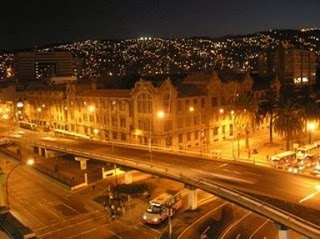
\includegraphics[width=0.6\linewidth]{Images/pucv.jpg} 
\caption{Edificio PUCV.}\label{fig:pucv}
\end{center}
\end{figure}
  \newpage

\section{Chapter 2}\label{sec:chap2}
  

\subsection{Tablas}

Los resultados se muestran en la tabla~\ref{table:resultados}...

\begin{table}[htbp!]
\begin{center}
\begin{tabular}{|l|l|l|l|l|l|l|l|}
\hline
Valores    & a & b & c & b & e  & f & g \\
\hline
Tipo 1     & 5 & 4 & 0 & 2 &  4 & 5 &  100  \\
Tipo 2     & 1 & 3 & 0 & 3 &  8 & 9 &  9  \\
Tipo 3     & 2 & 2 & 1 & 0 &  7 & 8 &  3  \\
Tipo 4     & 6 & 2 & 1 & 0 &  5 & 8 &  2  \\
\hline
\end{tabular}
\end{center}
\caption{Resultados\label{table:resultados}}
\end{table}

\subsection{Ecuaciones}

La ecuación~\ref{ec:smoothing-1} muestra...

\begin{equation} \label{ec:smoothing-1}
 {f_i}_1 (S_j) = x_{0}
\end{equation} 


\begin{equation} \label{ec:smoothing-2}
 {f_i}_n (S_j) =  x_{n-1} + \beta_i {f_i}_{n-1} (S_j)
\end{equation} 
  \newpage

  \section{Chapter 3}\label{sec:chap3}
  
% Please add the following required packages to your document preamble:

% Note: It may be necessary to compile the document several times to get a multi-page table to line up properly
\begin{longtable}{|l|l|l|l|l|l|}
    \hline
    \textbf{ID} &
      \textbf{Definición del   problema} &
      \textbf{Comentarios/Explicaciones} &
      \textbf{Ejemplos de   ocurrencia} &
      \textbf{\begin{tabular}[c]{@{}l@{}}Heurística   \\ incumplida\end{tabular}} &
      \textbf{\begin{tabular}[c]{@{}l@{}}Imágenes   \\ explicativas\end{tabular}} \\ \hline
    \endfirsthead
    %
    \multicolumn{6}{c}%
    {{\bfseries Table \thetable\ continued from previous page}} \\
    \hline
    \textbf{ID} &
      \textbf{Definición del   problema} &
      \textbf{Comentarios/Explicaciones} &
      \textbf{Ejemplos de   ocurrencia} &
      \textbf{\begin{tabular}[c]{@{}l@{}}Heurística   \\ incumplida\end{tabular}} &
      \textbf{\begin{tabular}[c]{@{}l@{}}Imágenes   \\ explicativas\end{tabular}} \\ \hline
    \endhead
    %
    P1 &
      inconsistent   language in content &
      the   used language in the web site is english and spanish when the expectation is   to keep only one at the time, otherwise will confuse the user &
      at   landing after selecting location &
      H4 &
      P1.png \\ \hline
    P2 &
      redundant   location selection &
      whenever   login is required and cancel to continue as a guest user, i have to select   every time the "Región" and "Comuna" &
      when   try to go to private zone (account) &
      H6 &
      \begin{tabular}[c]{@{}l@{}}P2.1.png\\ P2.2.png\end{tabular} \\ \hline
    P3 &
      Product   image sizes &
      Product   images at PLP or SLP are very small, compared with competitors Product images   should look bigger at this stage of purchase flow, so it´s breaking external   standard at this topic &
      go   to any PLP or SLP &
      H4 &
      P3.png \\ \hline
    P4 &
      Inconsistent   Terminology &
      when   looking at PDP price shows that is per piece, and packaging shows is per unit &
      inside   jumbo store go to glasses aisle and select any product, will show as P4.png   image &
      H4 &
      P4.png \\ \hline
    P5 &
      aesthetic   issue at related products section on PDP &
      on   the related products from PDP when sliding to right the first product of the   list is blocked by the hitbox of the slide back button &
      Go   to any PDP with related product list &
      H5 &
      P5.png \\ \hline
    P6 &
      Long   descriptions doesn´t look natural &
      On   some PDP where long description is there, this information should be   organized in a proper way &
      select   pc factory store, then go to this product: "Apple · Cargador (Adaptador)   de casa 20W USB C sin cable SEC" and select read more on PDP &
      H2 &
      P6.png \\ \hline
    P7 &
      No   feedback when adding product to cart &
      there   is no explicit feedback when a product is added to the cart, confirmation or   error message not coming &
      Go   to any PLP or SLP and add a product to the cart from there &
      H1 &
      P7.png \\ \hline
    P8 &
      Help   section not accessible for guest users &
      eventhought   help section exists is only accessible from "account" section which   requires that user is logged in &
      Find   help section as guest &
      H10 &
      P8.png \\ \hline
    P9 &
      Navigation   issue/flow issue &
      \begin{tabular}[c]{@{}l@{}}when   trying to achieve a goal the steps should\\ be clear and significant   irrespective if user is going\\ or coming back\end{tabular} \\ \hline &
      in   the checkout flow when adding a payment method the context is left to a third   party site, when user comes back without adding a credit card then, is coming   back to a different section (account) of the web site &
      H1,   H3, H7 &
      \begin{tabular}[c]{@{}l@{}}P9.1.png\\ P9.2.png\\ P9.3.png\\ P9.4.png\\ P9.5.png\end{tabular} \\ \hline
    P10 &
      Product   name and price missing from related products &
      Product   name and price are missing from related products at PDP &
      go   to any PDP with related product list, and watch at related product list &
      H2 &
      P10.png \\ \hline
    P11 &
      Profile   image is requested. &
      profile   image is required but useless for any functionality within the web site. &
      Go   to account -\textgreater information and password, watch that profile image is required &
      H8 &
      P11.png \\ \hline
    P12 &
      Tittle   not matching with selected option &
      the   tittle should be same or similar to the option selected &
      Go   to account -\textgreater information and password, watch that title is not same as selected option &
      H1 &
      \begin{tabular}[c]{@{}l@{}}P12.1.png\\ P12.2.png\end{tabular} \\ \hline
    P13 &
      Confusing save action &
      there is inconsistency between the screen save action and upload a picture, when user do upload a picture this is saved immediately to the profile and there   is no way to undo that action, apart of this the save action of the screen is   useless &
      Go to account -\textgreater information and password -\textgreater{}Execute the upload photo   feature &
      H3, H4 &
      P13.png \\ \hline
    P14 &
      Price mismatch at order summary &
      there is a mismatch in the sum of all the items and the details shown at order summary, expectation is that the tips are added to the order summary &
      During checkout flow select tips for shopper, whatch that is not reflected in final   amount &
      H2 &
      P14.png \\ \hline
    P15 &
      Incomplete feature &
      there   is a functionality option which is not understandable how it works as there is no functionality to add a membership under that context &
      Go   to account -\textgreater Memberships &
      H7 &
      \begin{tabular}[c]{@{}l@{}}P15.1.png\\      P15.2.png\end{tabular} \\ \hline
    \end{longtable}
  \newpage

  \section{Chapter 4}\label{sec:chap4}
  \input{Chapters/chapter_4.tex}
  \newpage

  \section{Conclusion}\label{sec:chap2}
  this are all the conclusions that you have found during your research
  \newpage
%%=============================================================================
%% Biblio

%\bibliographystyle{plain}
\bibliographystyle{alpha}
\bibliography{bibliography}	


\end{document}